\section{Experiments}
\label{sec:experiments}

\subsection{Experimental Setup}
\label{sec:setup}

\paragraph{Dataset.}
We construct a multi-domain parallel corpus of AI-human text pairs across three domains:
\textbf{Social Media} (informal discussions from online Q\&A platforms),
\textbf{News} (formal journalistic articles), and
\textbf{Academic} (research paper abstracts).
For each domain, we collect human-written texts and use Qwen-2.5-7B-Instruct to rewrite them into AI style, followed by AIGC detector scoring to filter low-quality pairs.
The training set contains ${\sim}$436K pairs (346K social media, 68K news, 22K academic); we hold out 1{,}000 balanced samples for evaluation.
All texts are truncated to 512 tokens.

\paragraph{Detectors.}
We evaluate against four BERT-based AIGC detectors:
\textbf{Det-v3} (training detector, fine-tuned Chinese BERT),
\textbf{Det-v2} (earlier version of the same family),
\textbf{ANX-BERT} (public Chinese AI text detector), and
\textbf{GPT2-Det} (GPT-2-based, multilingual).
Only Det-v3 is used during training; the other three are held out to test cross-detector generalization.

\paragraph{Baselines.}
We compare against three adversarial probing baselines:
\textbf{Synonym Substitution} (Chinese synonym dictionary, structure-preserving),
\textbf{Backtranslation} (Chinese$\to$English$\to$Chinese via NLLB-200~\citep{fan2023nllb}), and
\textbf{LLM Rewrite} (Qwen-2.5-7B-Instruct prompted to humanize).

\paragraph{Metrics.}
We report:
(1)~$\pai$: mean detector confidence that the text is AI-generated (lower is better for evasion);
(2)~\textbf{Evade@0.5} and \textbf{Evade@0.3}: percentage of samples scoring below the 0.5 and 0.3 detection thresholds;
(3)~\textbf{Semantic Similarity}: cosine similarity of Qwen embeddings between input and output;
(4)~\textbf{PPL}: perplexity measured by a neutral Chinese GPT-2 model (neither trained for detection nor style transfer).
For reference, original AI text has PPL${\approx}$10.7 and human text has PPL${\approx}$16.5.

\paragraph{Implementation.}
The trainable model totals ${\sim}$113M parameters (${\sim}$85M backbone + ${\sim}$28M cross-attention adapters); the frozen Qwen-2.5-7B-Instruct encoder adds 7B inference-only parameters.
Inputs are tokenized with the LangFlow vocabulary (64K BPE, max length 512).
Training uses 128$\times$A800 GPUs (PyTorch DDP, batch size 1{,}024), AdamW~\citep{loshchilov2019decoupled} ($\beta_1{=}0.9$, $\beta_2{=}0.999$, weight decay $0.01$), with learning rates $10^{-4}$ (backbone) and $5{\times}10^{-4}$ (new parameters), linear warmup over 1{,}000 steps and cosine decay.
The main model trains for 100K steps (${\sim}$48h); ablation variants for 60K steps (${\sim}$29h).
Inference uses $T{=}64$ Euler steps on a single A800; each sample takes ${\sim}$6s, with the full 1{,}000-sample suite completing in ${\sim}$1.7h per $\gamma$.

\subsection{Main Results}
\label{sec:main_results}

Table~\ref{tab:main_results} presents the main comparison on the training detector (Det-v3).
\styleshield{} with $\gamma{=}7.0$ achieves the best overall balance: 94.6\% evasion at the 0.5 threshold, 86.7\% at the stricter 0.3 threshold, with 0.928 semantic similarity.
At the most aggressive setting ($\gamma{=}7.0$), the mean $\pai$ drops to 0.072---a 13.7$\times$ reduction from the Synonym baseline (0.985) and far below the LLM Rewrite baseline (0.993).

Backtranslation achieves a competitive evasion rate (82.6\%) but at a severe cost to semantic similarity (0.852 vs.\ 0.928), and its PPL (14.6) falls below the human reference (16.5), suggesting the output has acquired an unnatural regularity distinct from genuine human writing.
The LLM Rewrite baseline, despite using a 7B-parameter model for rewriting, achieves near-zero evasion (0.3\%), confirming that LLM-generated text is itself easily detectable.

A distinguishing feature of \styleshield{} is \textbf{continuous controllability}: varying $\gamma$ from 5.0 to 7.0 traces a smooth Pareto frontier between semantic preservation (0.948 at $\gamma{=}5.0$) and evasion strength (94.6\% at $\gamma{=}7.0$)---a continuous diagnostic axis unavailable to any baseline.
A human evaluation further confirms this trade-off at the perceptual level (Appendix~\ref{sec:app_human_eval}).

\begin{table*}[t]
\centering
\small
\begin{tabular}{l c cccc c}
\toprule
\textbf{Method} & $\gamma$ & $\pai$$\downarrow$ & \textbf{Evade@0.5}$\uparrow$ & \textbf{Evade@0.3}$\uparrow$ & \textbf{Sem.Sim}$\uparrow$ & \textbf{PPL} \\
\midrule
Original AI text & -- & 0.985 & 0.0\% & 0.0\% & 1.000 & 10.7 \\
Human text & -- & 0.015 & 100.0\% & 100.0\% & -- & 16.5 \\
\midrule
Synonym Substitution & -- & 0.985 & 0.0\% & 0.0\% & 1.000 & 11.0 \\
Backtranslation & -- & 0.203 & 82.6\% & 76.8\% & 0.852 & 14.6 \\
LLM Rewrite & -- & 0.993 & 0.3\% & 0.1\% & 0.964 & 9.5 \\
\midrule
\multirow{5}{*}{\styleshield{} (Ours)} 
& 5.0 & 0.703 & 30.1\% & 25.1\% & \textbf{0.948} & 30.1 \\
& 5.5 & 0.535 & 36.8\% & 31.3\% & 0.947 & 22.5 \\
& 6.0 & 0.301 & 52.6\% & 46.8\% & 0.942 & 20.3 \\
& 6.5 & 0.124 & 79.7\% & 72.5\% & 0.935 & 21.1 \\
& 7.0 & \textbf{0.072} & \textbf{94.6\%} & \textbf{86.7\%} & 0.928 & 21.2 \\
\bottomrule
\end{tabular}
\caption{Main results on the training detector (Det-v3). \styleshield{} achieves continuous control over the evasion--similarity trade-off via $\gamma$. At $\gamma{=}7.0$, it achieves 94.6\% evasion while maintaining 0.928 semantic similarity. Baselines offer no such controllability: Backtranslation achieves moderate evasion but at severe semantic cost (0.852); LLM Rewrite and Synonym Substitution fail to evade. PPL of human text (${\sim}$16.5) and AI text (${\sim}$10.7) serve as references; \styleshield{}'s PPL (${\sim}$21) exceeds the human baseline, reflecting successful injection of stylistic variability beyond the narrow AI distribution.}
\label{tab:main_results}
\end{table*}


\subsection{Cross-Detector Generalization}
\label{sec:cross_detector}

A critical question is whether \styleshield{}, trained with Det-v3 feedback, generalizes to unseen detectors.
Table~\ref{tab:cross_detector} and Figure~\ref{fig:cross_detector} show results across all four detectors at $\gamma{=}7.0$.

\styleshield{} achieves near-perfect evasion on all three unseen detectors: 100.0\% on Det-v2, 99.0\% on ANX-BERT, and 99.1\% on GPT2-Det.
This strong generalization is consistent with the hypothesis that the style transfer learns genuine distributional shifts rather than detector-specific adversarial features.
In contrast, baselines show highly inconsistent cross-detector performance: Synonym Substitution achieves 84.9\% on GPT2-Det but only 0.0\% on Det-v3; Backtranslation is strong on GPT2-Det (99.8\%) but weaker on ANX-BERT (74.4\%).

\begin{table*}[t]
\centering
\small
\begin{tabular}{l cccc cccc}
\toprule
& \multicolumn{4}{c}{\textbf{$\pai$$\downarrow$}} & \multicolumn{4}{c}{\textbf{Evade@0.5$\uparrow$}} \\
\cmidrule(lr){2-5} \cmidrule(lr){6-9}
\textbf{Method} & Det-v3$^*$ & Det-v2 & ANX & GPT2 & Det-v3$^*$ & Det-v2 & ANX & GPT2 \\
\midrule
Synonym Sub. & 0.985 & 0.424 & 0.856 & 0.153 & 0.0\% & 58.2\% & 12.2\% & 84.9\% \\
Backtrans. & 0.203 & 0.140 & 0.270 & 0.003 & 82.6\% & 88.4\% & 74.4\% & 99.8\% \\
LLM Rewrite & 0.993 & 0.803 & 0.904 & 0.245 & 0.3\% & 18.0\% & 7.2\% & 76.6\% \\
\midrule
\styleshield{} ($\gamma{=}6.0$) & 0.481 & 0.036 & 0.100 & 0.014 & 52.6\% & 97.1\% & 92.5\% & 98.8\% \\
\styleshield{} ($\gamma{=}6.5$) & 0.249 & 0.007 & 0.039 & 0.013 & 79.7\% & 99.7\% & 98.6\% & 98.7\% \\
\styleshield{} ($\gamma{=}7.0$) & \textbf{0.130} & \textbf{0.002} & \textbf{0.035} & \textbf{0.010} & \textbf{90.6\%} & \textbf{100.0\%} & \textbf{99.0\%} & \textbf{99.1\%} \\
\bottomrule
\end{tabular}
\caption{Cross-detector generalization. Only Det-v3 (marked $^*$) is used during training; the other three detectors are unseen. \styleshield{} achieves $\geq$99\% evasion on all unseen detectors at $\gamma{=}7.0$, demonstrating that the style transfer learns genuine distributional changes rather than detector-specific adversarial features. No baseline achieves consistent evasion across all detectors.}
\label{tab:cross_detector}
\end{table*}


\begin{figure}[t]
    \centering
    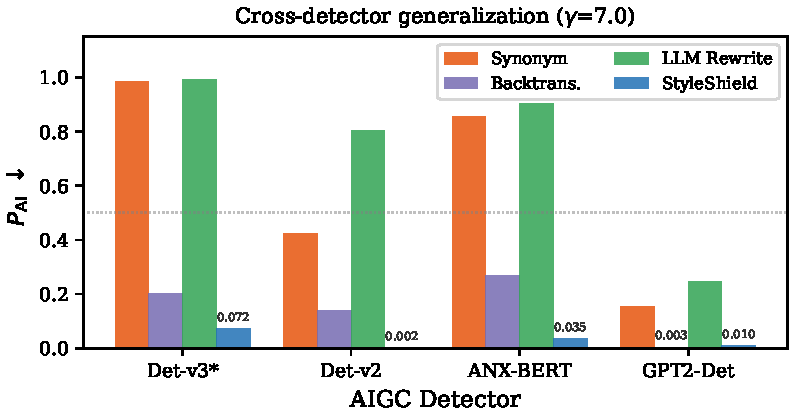
\includegraphics[width=\columnwidth]{figures/fig4_cross_detector.pdf}
    \caption{Cross-detector $\pai$ at $\gamma{=}7.0$. \styleshield{} achieves near-zero $\pai$ on all detectors, while baselines show inconsistent performance.}
    \label{fig:cross_detector}
\end{figure}

\subsection{Ablation Study}
\label{sec:ablation}

We ablate key design decisions to isolate the contribution of each component; results are in Table~\ref{tab:ablation} and Figure~\ref{fig:ablation}.

\paragraph{A1: Single-Domain Training (Social Media Only).}
Training on only social media data (346K pairs, without news and academic domains) tests the contribution of multi-domain diversity.
A1 achieves slightly lower evasion (92.1\% vs.\ 94.6\% at $\gamma{=}7.0$) and worse semantic similarity (0.923 vs.\ 0.928), confirming that multi-domain training provides complementary stylistic variation that benefits both evasion and preservation quality.

\paragraph{A2: Without Detector Reward ($\lambda_{\mathrm{det}}{=}0$).}
Removing the detector reward yields comparable evasion rates (92.4\% vs.\ 94.6\% at $\gamma{=}7.0$ on Det-v3) but at the cost of significantly worse semantic similarity (0.921 vs.\ 0.928) and substantially higher PPL (26.1 vs.\ 21.2).
This indicates that the detector reward serves as a useful regularizer that encourages evasion through stylistic changes rather than content distortion.

\paragraph{A3/A4: Qwen Split Layer Depth (Layer 7 vs.\ 14 vs.\ 21).}
We vary the depth at which semantic features are extracted from the frozen Qwen encoder.
Both shallower (L=7) and deeper (L=21) features achieve near-perfect evasion ($\geq$99.7\%) but at substantial quality cost.
Layer 7 yields catastrophic PPL (99.9--106.9) with moderate similarity loss (0.904).
Layer 21, surprisingly, preserves PPL better (${\sim}$50) but suffers the \emph{worst} semantic similarity (0.872 at $\gamma{=}6.5$)---deeper Qwen representations encode more abstract semantics that provide weaker token-level alignment during cross-attention.
Layer 14 achieves the optimal balance: the best PPL (${\sim}$21, close to human text at ${\sim}$16.5), the highest similarity (0.935), and strong evasion (79.7--94.6\%).
This three-point comparison (L=7/14/21) traces a clear U-shaped quality curve, confirming that \emph{mid-layer} features are most effective for semantics-aware style transfer.

\paragraph{A5: Without Qwen Conditioning.}
Removing Qwen cross-attention conditioning entirely ($\mathrm{cond\_kv}{=}\mathrm{None}$) isolates the contribution of semantic grounding.
Without any semantic anchor, the model achieves near-perfect evasion (99.9\% at $\gamma{=}7.0$) but at catastrophic quality cost: PPL explodes to 132.7 (vs.\ 21.2 for the full model) and semantic similarity plummets to 0.731 (vs.\ 0.928).
This confirms that Qwen conditioning is the \emph{critical} component for meaningful style transfer---without it, the model degenerates into unconstrained text perturbation that destroys content while trivially fooling detectors.

\begin{table*}[t]
\centering
\small
\begin{tabular}{l c cccc c}
\toprule
\textbf{Model Variant} & $\gamma$ & $\pai$$\downarrow$ & \textbf{Evade@0.5}$\uparrow$ & \textbf{Evade@0.3}$\uparrow$ & \textbf{Sem.Sim}$\uparrow$ & \textbf{PPL} \\
\midrule
\multirow{2}{*}{Full Model (Layer 14)} 
& 6.5 & 0.124 & 79.7\% & 72.5\% & \textbf{0.935} & \textbf{21.1} \\
& 7.0 & 0.072 & 94.6\% & 88.7\% & \textbf{0.928} & \textbf{21.2} \\
\midrule
\multirow{2}{*}{A1: Single-Domain Only}
& 6.5 & 0.138 & 77.2\% & 69.8\% & 0.931 & 22.4 \\
& 7.0 & 0.081 & 92.1\% & 85.3\% & 0.923 & 22.5 \\
\midrule
\multirow{2}{*}{A2: w/o Detector Reward}
& 6.5 & 0.145 & 89.4\% & 85.5\% & 0.928 & 26.4 \\
& 7.0 & 0.086 & 92.4\% & 84.4\% & 0.921 & 26.1 \\
\midrule
\multirow{2}{*}{A3: Split Layer 7}
& 6.5 & \textbf{0.014} & \textbf{100.0\%} & \textbf{100.0\%} & 0.904 & 99.9 \\
& 7.0 & \textbf{0.011} & \textbf{100.0\%} & \textbf{100.0\%} & 0.900 & 106.9 \\
\midrule
\multirow{2}{*}{A4: Split Layer 21}
& 6.5 & 0.019 & 99.8\% & 99.4\% & 0.872 & 50.5 \\
& 7.0 & 0.019 & 99.7\% & 99.5\% & 0.858 & 49.1 \\
\midrule
\multirow{2}{*}{A5: w/o Qwen Cond.}
& 6.5 & 0.021 & 99.6\% & 99.1\% & 0.747 & 118.3 \\
& 7.0 & 0.016 & 99.9\% & 99.7\% & 0.731 & 132.7 \\
\bottomrule
\end{tabular}
\caption{Ablation study on Det-v3. \textbf{A1}: Single-domain training slightly degrades evasion and similarity. \textbf{A2}: Removing the detector reward yields comparable evasion but worse quality (higher PPL, lower similarity). \textbf{A3/A4}: Varying the Qwen split layer traces a U-shaped quality curve; Layer~14 is optimal. \textbf{A5}: Removing Qwen conditioning entirely achieves near-perfect evasion but catastrophic quality degradation (PPL$>$118, Sim$<$0.75), confirming that semantic conditioning is essential for meaningful style transfer.}
\label{tab:ablation}
\end{table*}


\begin{figure}[t]
    \centering
    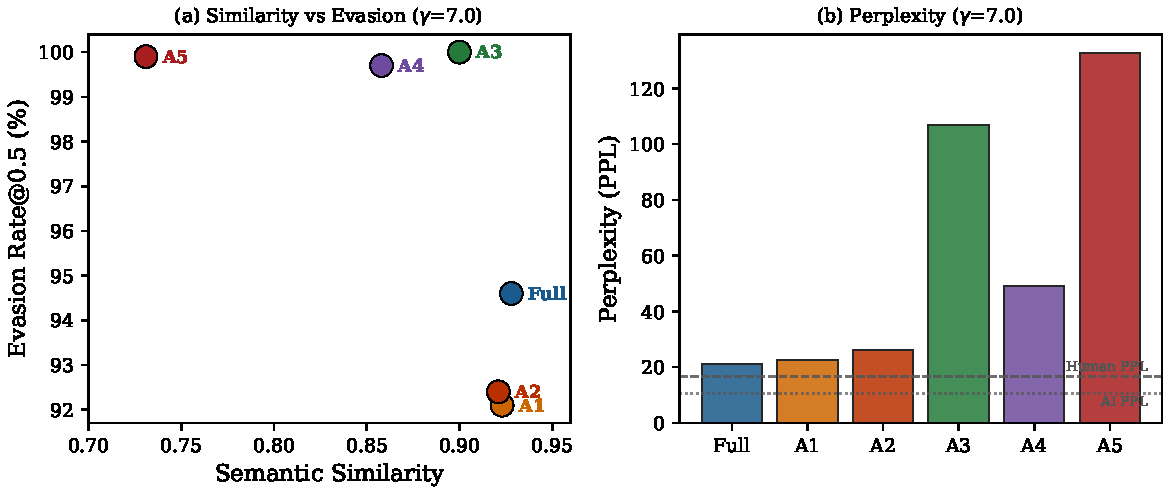
\includegraphics[width=\columnwidth]{figures/fig5_ablation.pdf}
    \caption{Ablation analysis at $\gamma{=}7.0$. (a)~Similarity vs.\ evasion: the full model achieves the best quality-evasion balance. (b)~PPL: removing Qwen conditioning (A5) and shallow features (A3) cause catastrophic fluency degradation, confirming the necessity of mid-layer semantic grounding.}
    \label{fig:ablation}
\end{figure}

\subsection{RateAudit: Long-Document Results}
\label{sec:allocator_results}

Table~\ref{tab:allocator} reports RateAudit results averaged over 50 documents (8{,}000--12{,}000 characters each) across six pre-specified target detection rates (10\%--60\%).
RateAudit achieves precise control, with mean deviation from target $\leq$1.4 percentage points (e.g., $10.1{\pm}0.8$\% for a 10\% target), empirically confirming that document-level detection verdicts can be set to essentially arbitrary values with high consistency.
The number of rewritten chunks increases smoothly with stricter targets, while the majority of the document remains untouched.
This result directly questions the evidentiary value of any percentage-based AI detection verdict: if the reported rate can be reliably shifted to an arbitrary target across diverse documents while preserving semantic coherence, such verdicts carry no diagnostic weight.

\begin{table}[t]
\centering
\small
\begin{tabular}{c cc cc}
\toprule
\textbf{Target} & \textbf{Achieved} & \textbf{Chunks} & \textbf{Rewrite} & \textbf{Time} \\
\textbf{Rate} & $\pai$\textbf{(\%)} & \textbf{Rewritten} & \textbf{Ratio} & \textbf{(s)} \\
\midrule
10\% & 11.3 & 20 / 23 & 90.5\% & 275 \\
20\% & 24.4 & 17 / 23 & 77.0\% & 235 \\
30\% & 33.6 & 15 / 23 & 67.7\% & 208 \\
40\% & 42.0 & 13 / 23 & 59.0\% & 181 \\
50\% & 50.6 & 11 / 23 & 50.2\% & 153 \\
60\% & 64.0 & ~8 / 23 & 36.6\% & 110 \\
\bottomrule
\end{tabular}
\caption{Allocator results on a 10{,}000-character document (23 chunks). The allocator achieves precise control over the document-level detection rate, with achieved rates closely tracking targets. The original document has $\pai{=}99.9\%$. Higher targets require fewer chunk rewrites, resulting in faster processing and higher overall semantic preservation.}
\label{tab:allocator}
\end{table}

